\documentclass[oneside,final,14pt]{extreport}
\usepackage[utf8]{inputenc}
\usepackage{pgfplots}
\documentclass{article}
\usepackage{listings}
\usepackage[russianb]{babel}
\usepackage{graphicx}
\lstset{extendedchars=\true}
\usepackage[14pt]{extsizes}
\usepackage{vmargin}
\usepackage{pb-diagram}
\DeclareGraphicsExtensions{.pdf,.png,.jpg}
\usepackage{proof}
\usepackage{minted}
\usepackage{amsfonts}
\usepackage{amsmath}
\renewcommand{\baselinestretch}{1.5}
\usepackage{amssymb}
\setpapersize{A4}
\setmarginsrb{1.5cm}{2cm}{2cm}{2cm}{0pt}{0mm}{0pt}{13mm}
\usepackage{indentfirst}
\usepackage{lscape}
\sloppy
\newcommand{\RNumb}[1]{\uppercase\expandafter{\romannumeral #1\relax}}
\begin{document}
% ! TEX root = book_part1.tex
\thispagestyle{empty}
~\vspace{-2cm}\setlength{\parindent}{0cm}
\begin{center}
		%\resizebox{!}{3cm}{\input{pingus.tex}}\\[2pt]
		\includegraphics{RTU.jpg}\\[2pt]
		\hrule{}\mbox{}\\[14pt]
		
		МИНОБРНАУКИ РОССИИ
		
		Федеральное государственное бюджетное образовательное учреждение\\
		высшего образования
		
		\textbf{<<МИРЭА – Российский технологический университет>>}
		
		\textbf{\large РТУ МИРЭА}
		\vfill	
		\textbf{\large Институт Кибернетики}
		
		\textbf{\large Курсовая работа}\\ по дисциплине\\ "Методы программирования"
		
		

		
		\large Тема курсовой работы\\ \textbf{Реализация шифратора на основе алгоритма ГОСТ 28147-89 в режие CBC}
		
		
\end{center}
\vfill
\begin{flushright}
\textbf{Выполнил:}


студент группы ККСО-04-19


Курбатов В.М.


\textbf{Научный руководитель:}


Кирюхин Виталий Александрович
\end{flushright}

	
	\vfill
	\begin{center}
	Москва --- 2021
	\end{center}



\tableofcontents
\newpage

\begin{center}



 \section*{Введение}
 \addcontentsline{toc}{section}{Введение}
 
 \end{center}

В данной курсовой работе представлена реализация ГОСТ 28147-89 (являющийся примером DES-подобных криптосистем, созданных по классической итерационной схеме Фейстеля)~- стандарт симметричного шифрования в режиме CBC(Cipher Block Chaining) - режим сцепления блоков шифротекста, на языке программирования С++ Алгоритм шифрования данных представляет собой 64-битовый блочный алгоритм с 256-битовым ключом.\\

Согласно извещению ФСБ о порядке использования алгоритма блочного шифрования ГОСТ 28147-89 данный алгоритм базового блочного шифрования применяется в криптографических методах обработки и защиты информации, не содержащей сведений, составляющих государственную тайну.

\newpage
 \begin{center}
\section{Теоретичекая часть}
 \end{center}


Клод Шеннон в ряде своих основополагающих работ по теории
шифрования сформулировал условия стойкости современного блоч­ного шифра. Такой шифр должен обладать свойствами перемеши­вания и рассеивания:\\



\begin{itemize}
\item рассеивание - это свойство шифра, при котором один символ
(бит) исходного текста влияет на несколько символов (битов) шифро­текста, оптимально - на все символы в пределах одного блока. Если
данное условие выполняется, то при шифровании двух блоков дан­ ных с минимальными отличиями между ними должны получаться
совершенно непохожие друг на друга блоки шифротекста. Точно
такая же картина должна иметь место и для зависимости шифро­
текста от ключа: один символ (бит) ключа должен влиять на
несколько символов (битов) шифротекста.
\end{itemize}



\begin{itemize}
\item перемешивание - это свойство шифра скрывать зависимостимежду символами исходного текста и шифротекста. Если шифр достаточно хорошо "перемешивает" биты исходного текста, то соответствующий шифротекст не содержит никаких статистических и
тем более функциональных закономерностей для стороннего наблю­дателя, обладающего лишь ограниченными вычислительными ресур­
сами.
\end{itemize}

\begin{center}
\subsection{Общие сведения о блочных шифрах}
 \end{center}


Характерной особенностью блочных криптоалгоритмов
является тот факт, что в ходе своей работы они осуществляют
преобразование блока входной информации фиксированной длины и
получают результирующий блок той же длины, но недоступный для
прочтения сторонним лицам, не владеющим ключом. \\


Таким образом,
схему работы блочного шифра можно описать функциями

\[Z = EnCrypt(X, Key)\]
и
\[X = DeCrypt(Z, Key)\]

Ключ $Key$ является параметром блочного криптоалгоритма и
представляет собой некоторый блок двоичной информации фикси­
рованного размера. Исходный $X$ и зашифрованный $Z$ блоки данных
также имеют фиксированную разрядность, равную между собой, но
необязательно равную длине ключа.\\


ГОСТ 28147-89 признан стойким алгоритмом.  Криптоалгоритм именуется идеально стойким, если зашифро­ванный блок данных можно прочесть только перебрав все возможные ключи, пока сообщение не окажется осмысленным. \\

Поскольку по теории вероятности искомый ключ будет найден с вероятностью $\frac{1}{2}$
после перебора половины всех ключей, постольку на взлом идеально
стойкого криптоалгоритма с ключом длиной $N$ потребуется в среднем $2^{N - 1}$. проверок. Таким образом, в общем случае стойкость блочного шифра зависит только от длины ключа и возрастает экспоненциально с ее ростом. \\


Характерным признаком блочных алгоритмов является много­ кратное и косвенное использование материала ключа. Это диктуется,
в первую очередь, требованием невозможности обратного декоди­
рования в отношении ключа при известных исходном и зашифро­
ванном текстах.\\


\subsection{Сеть Фейстеля}

Приведем описание сети Фейстеля, опираясь на [9]. Сеть Фейстеля получила широкое распро­странение, поскольку обеспечивает выполнение требования о много­ кратном использовании материала ключа и исходного блока
информации.\\

Классическая сеть Фейcтеля имеет структуру, представленную
на рис.1 

\begin{figure}[h]
\center{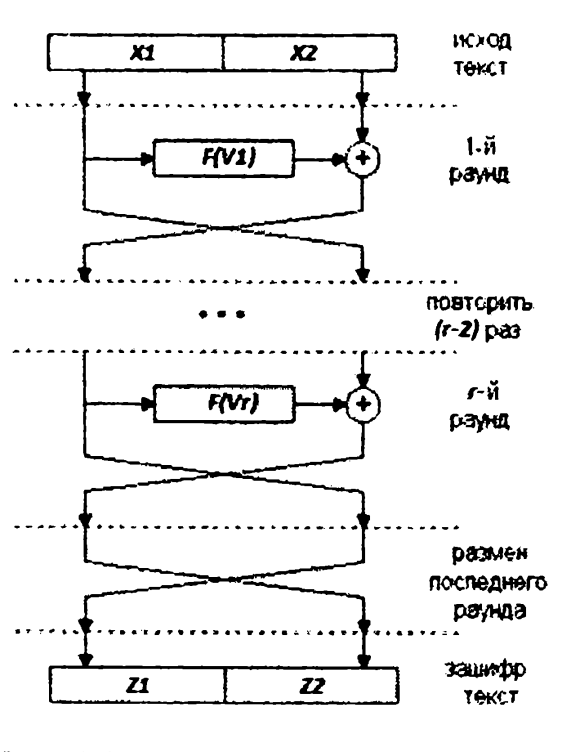
\includegraphics[width=0.6\textwidth]{1.png}}

\caption{Классическая сеть Фейстеля}
\end{figure}



Независимые потоки информации, появляющиеся из исходного блока, называются ветвями сети. В классической схеме их две. \\

Величины $V_{i}$, именуются параметрами сети, обычно это функции от материала ключа. Функция F является образующей. Действие,
состоящее из однократного вычисления образующей функции и
последующего наложения ее результата на другую ветвь с обменом
их местами, называется циклом или раундом (англ. round) сети
Фейcтеля. \\


Оптимальное число раундов $K - 8-32$. Важно то, что
увеличение количества раундов значительно увеличивает крипто­
стойкость любого блочного шифра к криптоанализу.\\


В современных алгоритмах обычно применяют модификацию
сети Фейcтеля для большего числа ветвей. Это в первую очередь
связано с тем, что при больших размерах кодируемых блоков (128 и
более битов) становится неудобно работать с математическими
функциями по модулю 64 и выше.\\



Сеть Фейcтеля надежно зарекомендовала себя как крипто­стойкая схема произведения преобразований, и ее можно найти
практически в любом современном блочном шифре. Незначительные
модификации касаются обычно дополнительных начальных и конеч­ных преобразований (англ. - whitening) шифруемого блока. Подобные
преобразования, выполняемые обычно также (исключающим или)  или сложением, имеют целью повысить начальную рандомизацию
входного текста. \\

Таким образом, криптостойкость блочного шифра,
использующего сеть Фейштеля, определяется на 95 \% функцией $F$ и
правилом вычисления $V_{i}$, из ключа.\\

\begin{center}
\subsection{ГОСТ 28147-89}
 \end{center}

В описываемом алгоритме блок длинной 64 бита, подлежащий зашифровыванию, разделяется на две равные части по 32 бита - правую и левую. Затем выполняется 32 итерации с использованием итерационных ключей, получаемых из исходного 256-битного ключа шифрования.


\begin{figure}[h!]
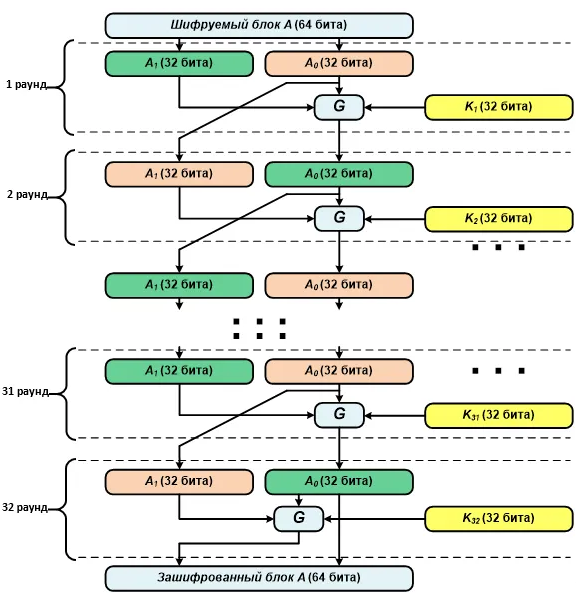
\includegraphics[width=0.9\textwidth]{2.png}
\caption{Схема работы алгоритма при зашифровывании}
\end{figure}


~\



Во время каждой итерации, кроме 32, с правой и левой половиной зашифровываемого блока производится одно преобразование, основанное на сети Фейстеля. Сначала правая часть складывается по модулю 32 с текущим итерационным ключом, затем полученное 32-битное число делится на восемь 4-битных и каждое из них с использованием таблицы перестановки преобразуется в другое 4-битное число (нелинейное биективное преобразование). \\

После этого преобразования полученное число циклически сдвигается влево на одиннадцать разрядов. Далее результат ксорится с левой половиной блока. Получившееся 32-битное число записывается в правую половину блока, а старое содержимое правой половины переносится в левую половину блока.\\

\begin{figure}[h!]
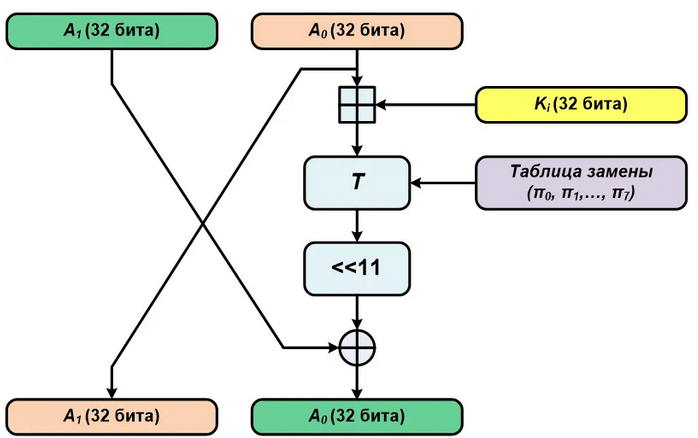
\includegraphics[width=0.9\textwidth]{3.png}
\caption{Схема одной итерации}

\end{figure}



~\




В ходе последней (тридцать второй) итерации так же, как описано выше, преобразуется правая половина, после чего полученный результат пишется в левую часть исходного блока, а правая половина сохраняет свое значение. 


Итерационные ключи получаются из исходного 256-битного ключа. Исходный ключ делится на восемь 32-битных подключей, и далее они используются в следующем порядке: три раза с первого по восьмой и один раз с восьмого по первый.\\

\begin{figure}[h!]
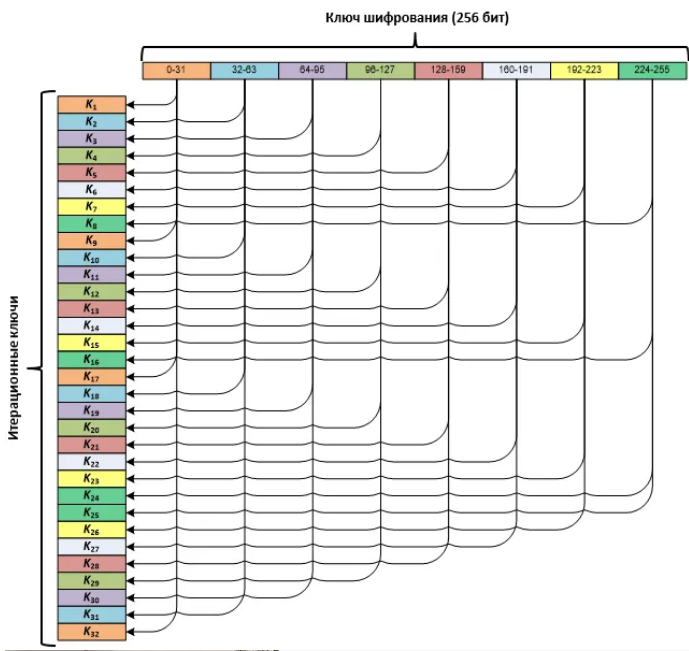
\includegraphics[width=1\textwidth]{4.png}
\caption{Схема получения итерационных ключей}

\end{figure}



~\



Для расшифровывания используется такая же последовательность итераций, как и при зашифровывании, но порядок следования ключей изменяется на обратный.\\


\begin{figure}[h!]
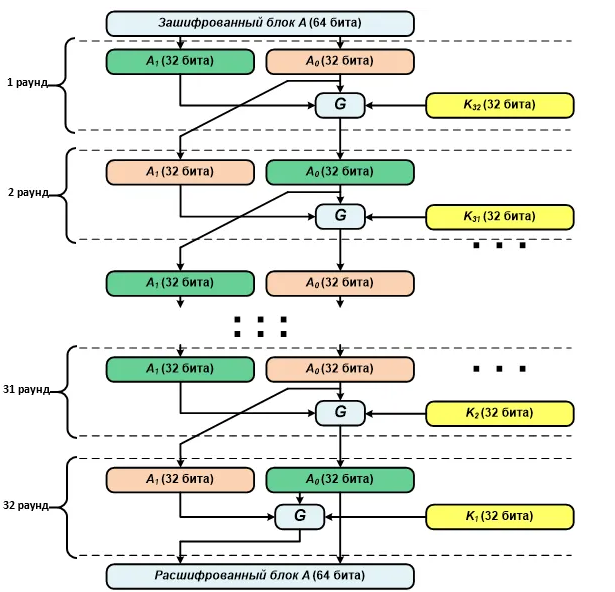
\includegraphics[width=0.9\textwidth]{5.png}
\caption{Схема работы алгоритма при расшифровывании}

\end{figure}



~\




Для шифровки исходного текста произвольной длины блочные
шифры могут быть использованы в нескольких режимах:\\

\begin{itemize}
\item электронной кодировочной книги (ЕСВ - Electronic Code
Book);
\item сцепления блоков шифрованного текста (СВС - Cipher
Block Chaining);
\item  обратной связи по шифрованному тексту (CFB - Cipher
Feedback);
\item обратной связи по выходу (OFB - Output Feedback).
\end{itemize}
\\


В режиме сцепления блоков шифрованного текста (СВС)
каждый блок исходного текста складывается поразрядно по модулю 2
с предыдущим блоком шифрованного текста, а затем шифруется. Для начала процесса шифрования используется синхропосылка (или начальный вектор), которая передается в канал
связи в открытом виде.\\

\begin{figure}[h!]
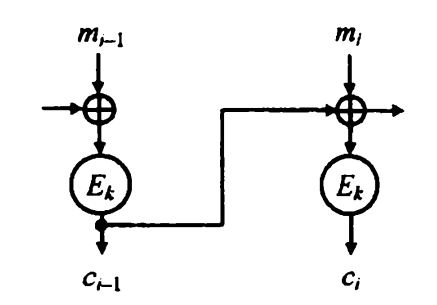
\includegraphics[width=0.4\textwidth]{6.png}
\caption{Режим сцепления блоков шифрованного текста}
\end{figure}




~\


\[c_{i} = E_{k}(m_{i}\oplus c_{i -1} )\]

и

\[m_{i} = D_{k}(c_{i})\oplus c_{i-1}\] 



То есть, схема работы при шифровании будет иметь вид:\\

\begin{figure}[h!]
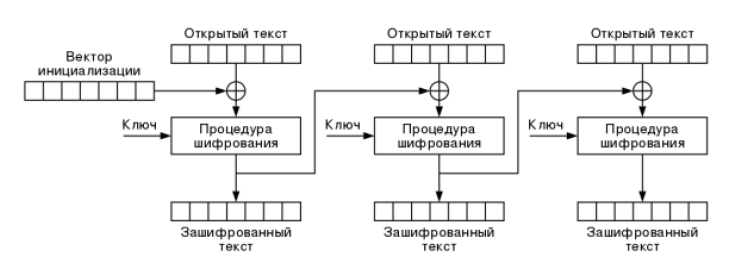
\includegraphics[width=1\textwidth]{7.png}
\caption{Схема работы при шифровании в режиме СВС}

\end{figure}




~\



А при расшифровании будет иметь вид:\\

\begin{figure}[h!]
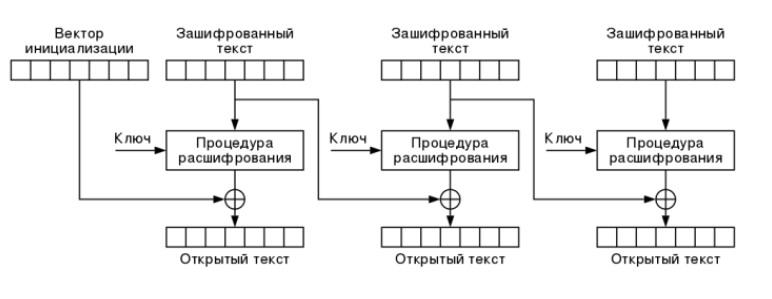
\includegraphics[width=1\textwidth]{8.png}
\caption{Схема работы при расшифровании в режиме СВС}

\end{figure}





~\


Стойкость режима СВС равна стойкости блочного шифра, лежа­щего в его основе. Кроме того, структура исходного текста скрыва­
ется за счет сложения предыдущего блока шифрованного текста с
очередным блоком открытого текста. Стойкость шифрованного
текста увеличивается, поскольку становится невозможной прямая
манипуляция исходным текстом, кроме как путем удаления блоков из
начала или конца шифрованного текста.\\



К недостаткам CBC стоит отнести возможность определения начала изменения данных по изменению шифротекста (если сравнить шифротексты двух сообщений с одним и тем же ключом, то номер первого блока, в котором шифротексты различаются, будет соответствовать номеру первого блока, в котором различаются исходные сообщения).\\


К достоинствам CBC стоит отнести:

\begin{itemize}
\item постоянная скорость обработки блоков (скорость определяется эффективностью реализации шифра; время выполнения операции «xor» пренебрежимо мало);

\item отсутствие статистических особенностей, характерных для режима ECB (поскольку каждый блок открытого текста «смешивается» с блоком шифротекста, полученным на предыдущем шаге шифрования);
\end{itemize}

\begin{center}
\subsection{Сравнительными характеристики методов шифровки блочных шифров}
 \end{center}
 
Приведу таблицу с сравнительными характеристиками методов шифровки блочных шифров:\\



\begin{tabular}{|p{5cm}|p{3cm}|p{3cm}|p{3cm}|p{3cm}|}
\hline 
Характеристика & ECB & CBC & CFB & OFB \\ 
\hline 
Блоки, от
которых зависит
шифрование
блока & Текущий & Все предыдущие & Все предыдущие & Позиция блока в файле \\ 
\hline 
Результат
искажения
одного бита при
передаче & Порча всего текущего блока & Порча всего текущего и всех последующих блоков & Порча одного бита текущего блока и всех последующих блоков & Порча одного бита текущего блока \\ 
\hline 
Возможность
кодирования без
дополнения
числа байтов, 
некратных блоку & Нет & Нет & Да & Да \\ 
\hline 
Поступление на выход криптосистемы & Выход криптоалгоритма & Выход криптоалгоритма & XOR-маска с исходным текстом & XOR-маска с исходным текстом \\ 
\hline 
\end{tabular} 



~\



\begin{center}
\section{Практическая часть}
 \end{center}



В тексте стандарта ГОСТ 28147-89 указывается, что поставка заполнения узлов замены (S-блоков) производится в установленном порядке, то есть разработчиком алгоритма.  \\


В своей реализации я использовал узел замены определленные документом RFC 4357. Идентификатор: id-Gost28147-89-CryptoPro-A-ParamSet. OID: 1.2.643.2.2.31.1.\\

\begin{figure}[h!]
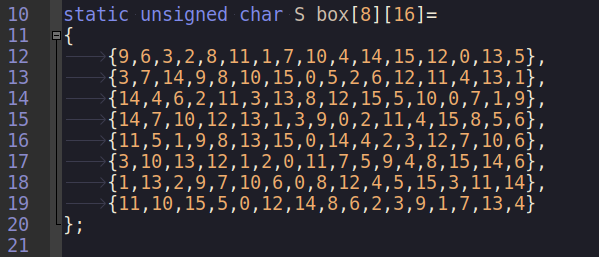
\includegraphics[width=0.6\textwidth]{9.png}
\caption{Таблица замены}
\end{figure}




~\



Данный узел замен используется криптопровайдером CryptoPRO CSP по умолчанию. Так же данный узел замен используется в ПО "Верба-О".

Далее опишу используемые мною функции:\\

$Add\_mod2$~- функция, реализующая сложение двух двоичных векторов по модулю 2. Каждый байт первого вектора $\oplus$ с соответствующим байтом второго вектора, результат операции записываем в третий вектор.\\

\begin{figure}[h!]
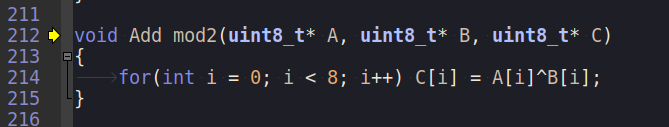
\includegraphics[width=0.9\textwidth]{10.png}
\caption{Функция $Add\_mod2$}
\end{figure}




~\



$add\_mod32$~- функция, реализующая сложение двух двоичных векторов по модулю 32. Два исходных 4-байтовых вектора представляются как два 32-битных числа и затем складываются. Если появляется переполнение - отбрасывается. \\

Стоит заметить, что данная функция аналогична сложению в кольце вычетов по модулю 2 в степени n.\\


\begin{figure}[hb!]
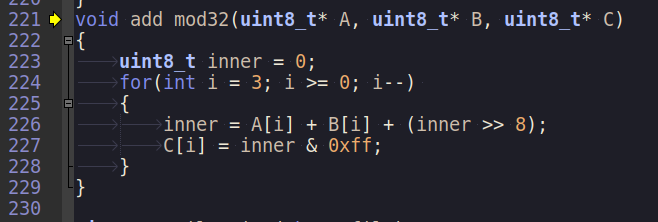
\includegraphics[width=0.9\textwidth]{11.png}
\caption{Функция $add\_mod32$}
\end{figure} \\


~\



$GOST\_28147\_89\_T$~- функция, выполняющая нелинейное биективное преобразование. Выполняется на основе таблицы подстановок в $S_box$ следующим образом: исходный
32-битный вектор разбивается на 4-х битные подпоследовательности, но- мер следования которых определяет строчку в таблице замен, а значение
номер индекса в этой ячейке, после чего значение в этой ячейке становится
значением 4-х битного вектора. В конце 4-х битные вектора складываются
обратно в 32-х битный. 


\begin{figure}[h]
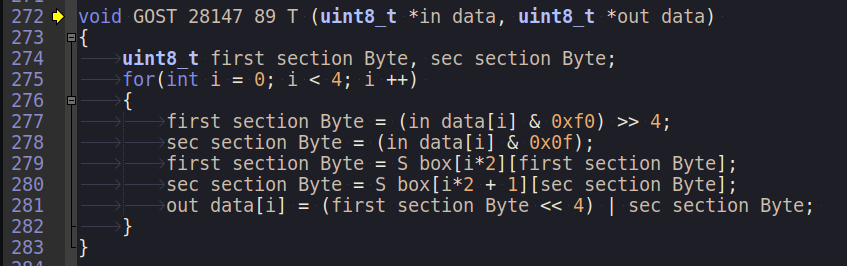
\includegraphics[width=1.1\textwidth]{12.png}
\caption{Функция $GOST\_28147\_89\_T$}
\end{figure}




~\



$GOST\_28147\_89\_g$~- функция, выполняющая преобразование $g$. Это преобразование включает
в себя сложение правой части блока с итерационным ключом по модулю
32, нелинейное биективное преобразование и сдвиг влево на одиннадцать
разрядов.


\begin{figure}[h!]
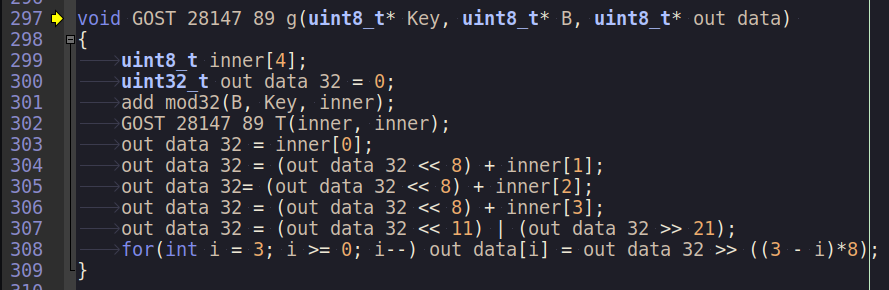
\includegraphics[width=1\textwidth]{13.png}
\caption{Функция $GOST\_28147\_89\_g$}
\end{figure}





~\



$GOST\_28147\_89\_G$~- функция, выполняющая преобразование $G$. Данное преобразование представляет собой одну итерацию цикла зашифровывания или расшифровывания
(с первой по тридцать первую). Включает в себя преобразование $g$,
сложение по модулю 2 результата преобразования $g$ с правой половиной блока и
обмен содержимым между правой и левой частью блока.\\

\begin{figure}[h!]
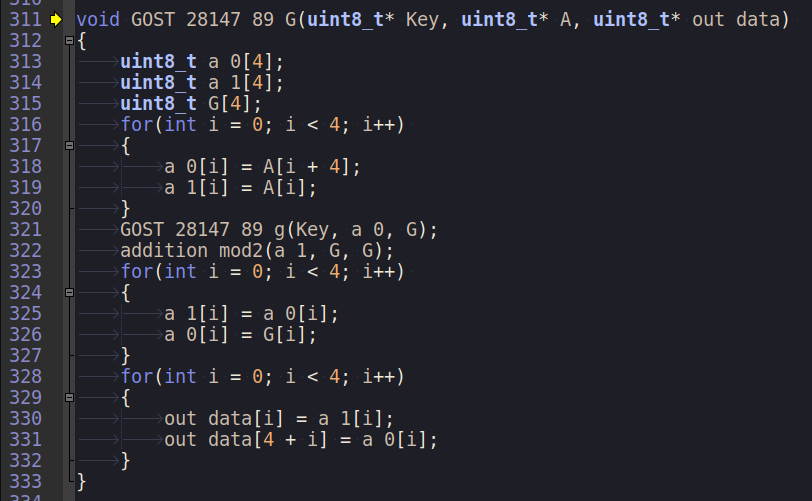
\includegraphics[width=1\textwidth]{14.png}
\caption{Функция $GOST\_28147\_89\_G$}
\end{figure}\\





~\


$GOST\_28147\_89\_G\_Finally$~- функция, выполняющая финальное преобразование $G$. Это последняя
(тридцать вторая) итерация цикла зашифровывания или расшифровывания. От простого преобразования $G$ отличается отсутствием обмена значениями между правой и левой частью исходного блока.\\

~\



\begin{figure}[h!]
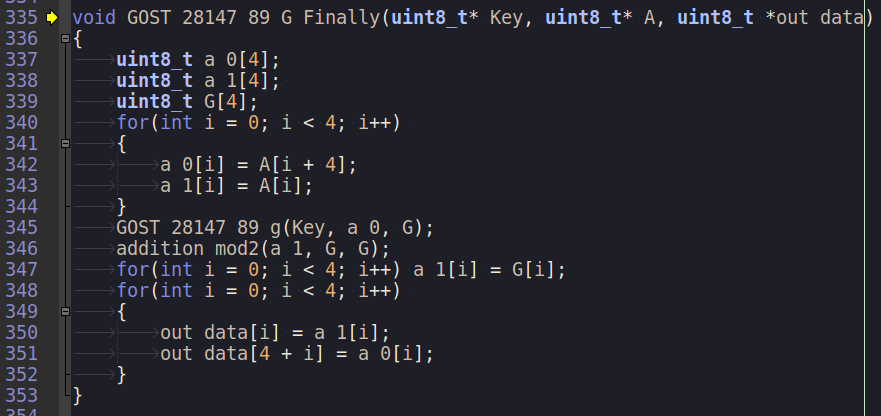
\includegraphics[width=0.9\textwidth]{15.png}
\caption{Функция $GOST\_28147\_89\_G\_Finally$}
\end{figure}




~\



$Produce\_IV$~- функция, отвечающая за синхропысылку$(IV)$.\\

\begin{figure}[h!]
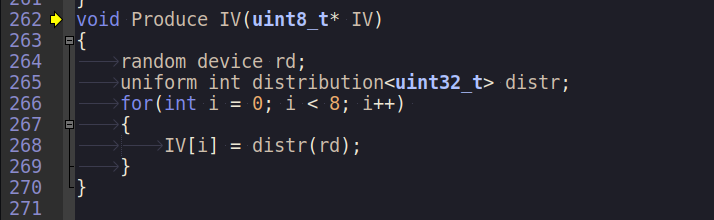
\includegraphics[width=0.9\textwidth]{16.png}
\caption{Функция IV}
\end{figure}





~\


$GOST\_28147\_89\_encrypt$~- функция, отвечающая за шифрование. Шифрование производится путем тридцати двух итераций, с первой по
тридцать первую с применением преобразования $G$ и тридцать вторую с
применением $G_Finally$.\\

\begin{figure}[h!]
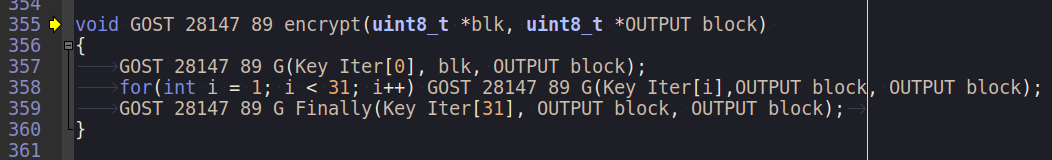
\includegraphics[width=1.1\textwidth]{17.png}
\caption{Функция шифрования}
\end{figure}




~\



$GOST\_28147\_89\_decrypt$~- функция, отвечающая за расшифрование. Расшифровыва-
ние выполняется аналогично зашифровыванию с использованием итераци-
онных ключей в обратном порядке.\\

\begin{figure}[h!]
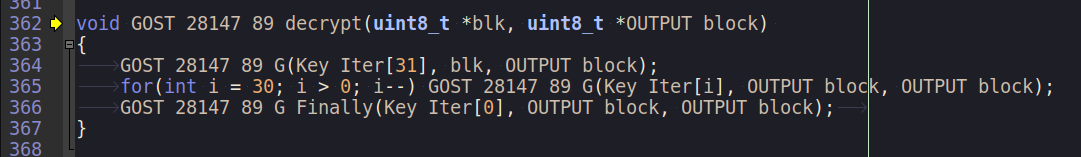
\includegraphics[width=1.1\textwidth]{18.png}
\caption{Функция расшифрования}
\end{figure}




~\



\subsection{Демонстрация работы программы}


Продемонстрируем работу программы.\\
Содержание файла $test.txt:$\\

\begin{figure}[h!]
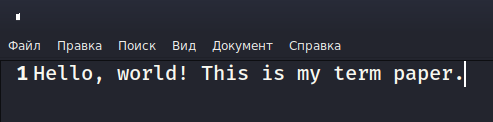
\includegraphics[width=0.4\textwidth]{19.png}
\caption{Соержание файла test.txt}
\end{figure}


После того, как я ввел файл, который необходимо зашифровать с созданием ключа, то в директории появились файлы $key.txt$ - созданный ключ, $ENCRYPTED.txt$ - зашифрованный текст.

\begin{figure}[h!]
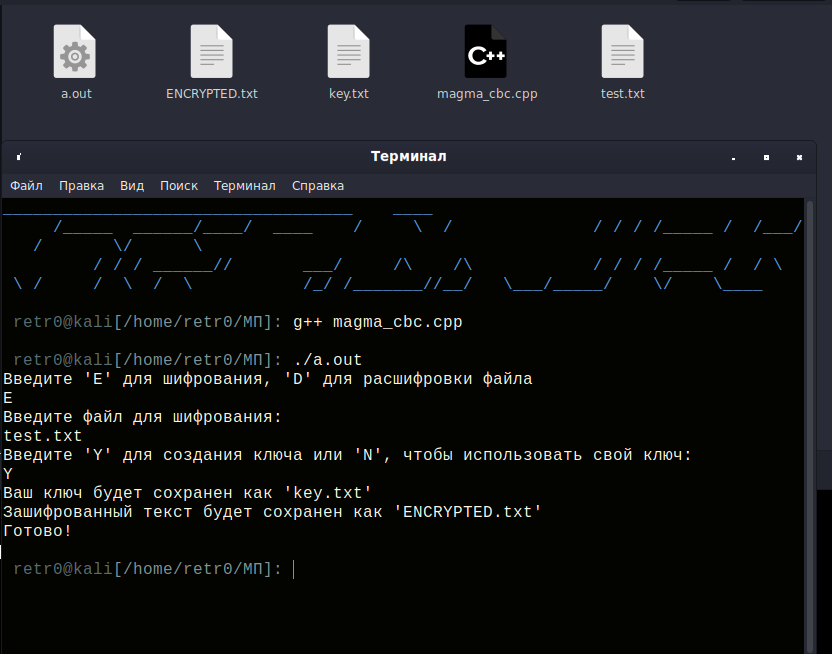
\includegraphics[width=1\textwidth]{20.png}
\caption{В директории появились файла key.txt и ENCRYPTED.txt }

\end{figure}


Содержание файла $ENCRYPTED.txt$:\\

\begin{figure}[h!]
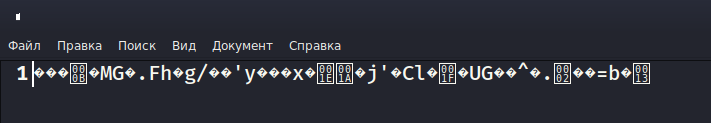
\includegraphics[width=0.8\textwidth]{21.png}
\caption{Содержание файла ENCRYPTED.txt }
\end{figure}


Затем попробуем расшифровать файл $ENCRYPTED.txt$, введя имя файла, содержащий ключ:\\

\begin{figure}[h!]
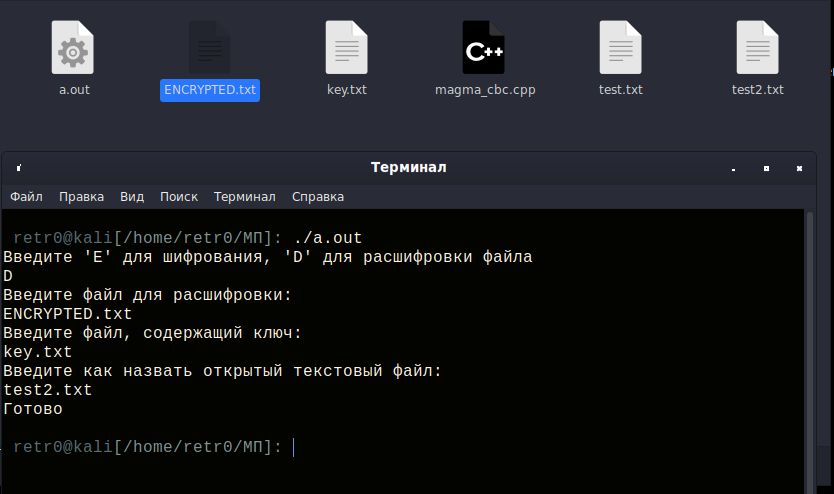
\includegraphics[width=0.9\textwidth]{22.png}
\caption{Расшифрование ENCRYPTED.txt }
\end{figure}


Видим, что появился файл $test\_2.txt$, откроем его:\\

\begin{figure}[h!]
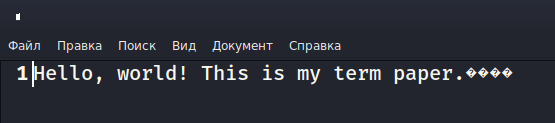
\includegraphics[width=0.8\textwidth]{23.png}
\caption{Результат расшифрования файла ENCRYPTED.txt }

\end{figure}



~\


\subsection{Тест скорости работы программы}

Проверим скорость работы алгоритма на примере шифрования 2 файлов размером $5MB$ и  $163MB$\\


Шифрование файла размером $1MB$:\\

\begin{figure}[h!]
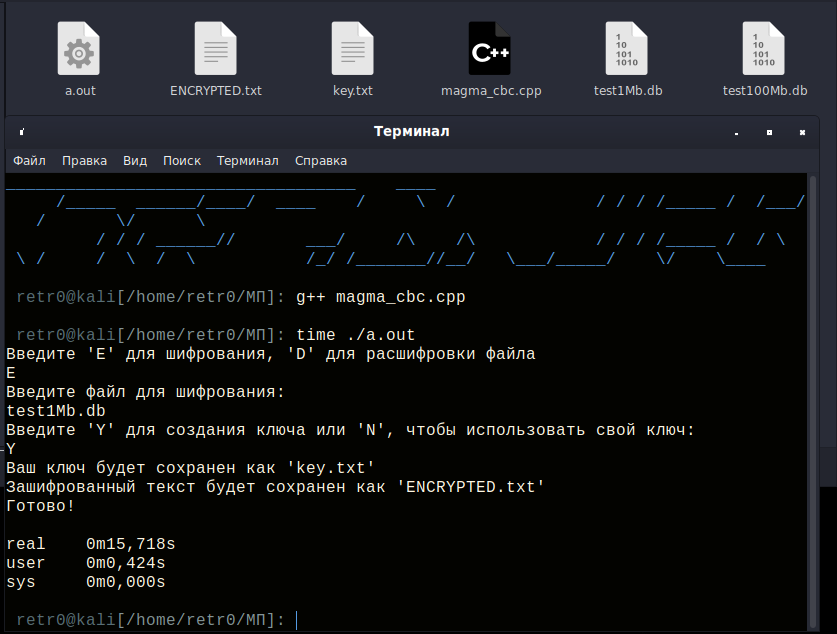
\includegraphics[width=1\textwidth]{24.png}
\caption{Шифрование файла размером 1MB}

\end{figure}



Шифрование файла, размером $100MB$:\\

\begin{figure}[h!]
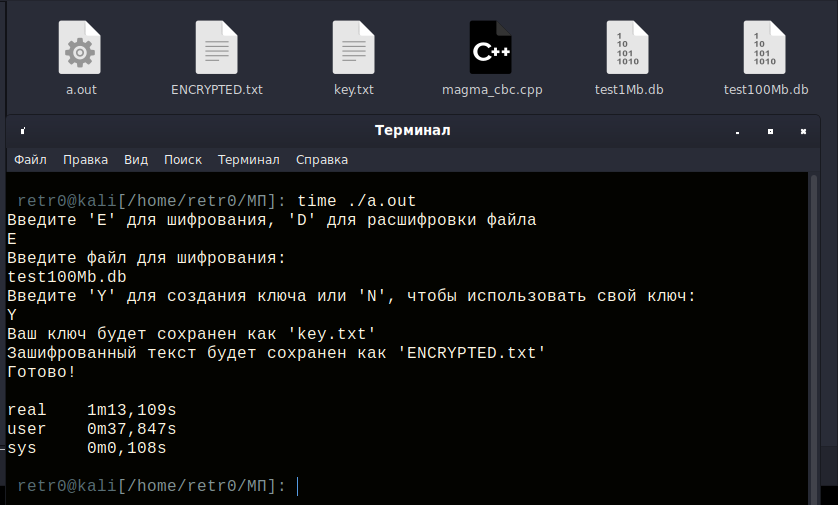
\includegraphics[width=1\textwidth]{25.png}
\caption{Шифрование файла размером 100MB}
\end{figure}


\newpage


\begin{center}
\section*{Заключение}
 \end{center}
\addcontentsline{toc}{section}{Заключение}

В данной работе я реализовал алгоритм шифрования ГОСТ $28147-89$, а также провел исследования скорости шифрования реализованного мной алгоритма. Шифр является устойчивым к атакам путем полного перебора.\\



\begin{thebibliography}{10}
\addcontentsline{toc}{section}{\bibname}

\bibitem{Gluxov}
Шнайер Б. – Прикладная криптография. Протоколы, алгоритмы
и исходные тексты на языке С – М.:Издательский дом «Вильямс» –
2016. – 1040 с.
\bibitem{Kurosh}
А. Б. Лось, А. Ю. Нестеренко, М. И. Рожков. – Криптографические
методы защиты информации: учебник для академического ба-
калавриата – 2-е изд., испр. – М. : Издательство Юрайт, 2018. – 473
с.
\bibitem{Liu4iu}
Панасенко С.П. – Алгоритмы шифрования. Специальный справоч-
ник. – СПб.: БХВ-Петербург, 2009. – 506 с.: ил.

\bibitem{Liweriu}

Popov, V., Kurepkin, I., and S. Leontiev. Additional Cryptographic Algorithms for Use with GOST 28147-89, GOST R 34.10-94, GOST R 34.10-2001, and GOST R 34.11-94 Algorithms (англ.) // RFC 4357. — IETF, January 2006.
\bibitem{Lweriu}
Романец Ю.В., Панасенко С.П., Заботин И.А., Петров С.В., Ракитин В.В., Дударев Д.А., Сырчин В.К., Салманова Ш.А. Глава 3. История создания алгоритма ГОСТ 28147-89 и принципы, заложенные в его основу // Фирма «АНКАД» – 25 лет на службе обеспечения информационной безопасности России (рус.) / под ред. Романца Ю.В.. — М.: Техносфера, 2016. — С. 9—19. — 256 с. — ISBN 978-5-94836-429-2.

\bibitem{weriu}

Саломаа А. Криптография с открытым ключом. - М., 1995.
\bibitem{LbdfLiu}

 Винокуров А. Алгоритм шифрования ГОСТ 28147-89, его использование и реализация для компьютеров платформы Intel x86.
\bibitem{LsdfLiu}

ГОСТ 28147-89. Системы обработки информации. Защита криптографическая. Алгоритм криптографического преобразования.
\bibitem{Libfiu}
Файстель Хорст. Криптография и компьютерная безопасность. Перевод А.Винокурова по изданию Horst Feistel. Cryptography and Computer Privacy, Scientific American, May 1973, Vol. 228, No. 5, pp. 15-23. 

\bibitem{Lbdwewwiu}

Информационная технология. Криптографическая защита информации. Функция хэширования ГОСТ Р34.11-94, Госстандарт РФ, М., 1994.

\newpage
\begin{center}
\section{Приложение}
 \end{center}

\textbf{Исходный код:}
	


\scriptsize{
\lstset{language=C++}          
\begin{lstlisting}                
#include <iostream>
#include <random>
#include <ctime>
#include <cmath>
#include <fstream>
#include <string>

using namespace std;

static unsigned char S_box[8][16]=
{
	{9,6,3,2,8,11,1,7,10,4,14,15,12,0,13,5},
	{3,7,14,9,8,10,15,0,5,2,6,12,11,4,13,1},
	{14,4,6,2,11,3,13,8,12,15,5,10,0,7,1,9},
	{14,7,10,12,13,1,3,9,0,2,11,4,15,8,5,6},
	{11,5,1,9,8,13,15,0,14,4,2,3,12,7,10,6},
	{3,10,13,12,1,2,0,11,7,5,9,4,8,15,14,6},
	{1,13,2,9,7,10,6,0,8,12,4,5,15,3,11,14},
	{11,10,15,5,0,12,14,8,6,2,3,9,1,7,13,4}
};


uint32_t File_Size(char*);
uint32_t Blocks(uint32_t);

static uint8_t Key[32];
static uint8_t Key_Iter[32][3];

void Add_mod2(uint8_t*, uint8_t*, uint8_t*);
void addition_mod2(uint8_t*, uint8_t*, uint8_t*);
void add_mod32(uint8_t*, uint8_t*, uint8_t*);

void Produce_key();
void Produce_IV(uint8_t*);

void GOST_28147_89_T(uint8_t*, uint8_t*);
void GOST_28147_89_Extend_Key(uint8_t[32][3]);
void GOST_28147_89_g(uint8_t*, uint8_t*, uint8_t*);
void GOST_28147_89_G(uint8_t*, uint8_t*, uint8_t*);
void GOST_28147_89_G_Finally(uint8_t*, uint8_t*, uint8_t*);
void GOST_28147_89_encrypt(uint8_t *, uint8_t*);
void GOST_28147_89_decrypt(uint8_t*, uint8_t*);


int main(int argc, char* argv[]) 
{
	char INPUT_DATA_1[32], INPUT_DATA_2[32], E, K, T = 'N'; 
	uint8_t Buff[8], Enc[8], IV[8];
	cout<<"Введите 'E' для шифрования, 'D' для расшифровки файла"<<endl;
	cin>>E;
	if(E == 'E') 
	{
		cout<<"Введите файл для шифрования: "<<endl;
		cin>>INPUT_DATA_1;
		ifstream fs(INPUT_DATA_1, ios_base::binary);
		while(!fs.is_open())
		{
			cout<<"Файл не существует. Пожалуйста, попробуйте еще раз: "<<endl;
			cin>>INPUT_DATA_1;
			fs.open(INPUT_DATA_1, ios_base::binary);
		}
		cout<<"Введите 'Y' для создания ключа или 'N', чтобы использовать свой ключ:"<<endl;
		cin>>K;
		if(K == 'Y') 
		{
			cout<<"Ваш ключ будет сохранен как 'key.txt'"<<endl;
			Produce_key();
		}
		else if(K == 'N')
		{
			cout<<"Введите свой ключ файл:"<<endl;
			cin>>INPUT_DATA_2;
			ifstream Key_file(INPUT_DATA_2, ios_base::binary);
			while(!Key_file.is_open())
			{
				cout<<"Что-то не так с вашим ключевым файлом. Пожалуйста, попробуйте еще раз: "<<endl;
				cin>>INPUT_DATA_2;
				Key_file.open(INPUT_DATA_2, ios_base::binary);
			}
			Key_file.read((char*)Key, 32);
			Key_file.close();
		}
		GOST_28147_89_Extend_Key(Key_Iter);
		Produce_IV(IV);
		
		cout<<"Зашифрованный текст будет сохранен как 'ENCRYPTED.txt'"<<endl;
		ofstream OUT("ENCRYPTED.txt" , ios_base::binary);
		
		for(int i = 0; i < 8; i++)
		{
			OUT<<IV[i];
		}
		uint8_t Buff[8];
		for(int i = 0; i < 8; i++)
		{
			Buff[i] = 0;
		}
		
		uint32_t size = File_Size(INPUT_DATA_1);
		uint32_t Blocks_32 = Blocks(size);
		int cursor = 0, temp = 8;
		for(int k = 0; k < Blocks_32; k++) 
		{
			if((cursor + temp) <= size) 
			{
				fs.read((char*)Buff, temp);
				Add_mod2(IV, Buff, IV);
				GOST_28147_89_encrypt(IV, IV);
				for(int i = 0; i < 8; i++) OUT<<IV[i];
				cursor += temp;
			}
			else 
			{
				temp = size - cursor;
				if(temp > 0) 
				{
					for(int i = 0; i < 8; i++) Buff[i] = 0;
					fs.read((char*)Buff, temp);
					Add_mod2(IV, Buff, IV);
					GOST_28147_89_encrypt(IV, IV);
					for(int i = 0; i < 8; i++) OUT<<IV[i]; 
				}
			}
		}
		fs.close();
		OUT.close();
		cout<<"Готово!"<<endl;
	}
	else if(E == 'D') 
	{
		cout<<"Введите файл для расшифровки: "<<endl;
		cin>>INPUT_DATA_1;
		ifstream CT(INPUT_DATA_1, ios_base::binary);
	
		while(!CT.is_open())
		{
			cout<<"Файл не найден. Пожалуйста, попробуйте еще раз: "<<endl;
			cin>>INPUT_DATA_1;
			CT.open(INPUT_DATA_1, ios_base::binary);
		}
		
		cout<<"Введите файл, содержащий ключ:"<<endl;
		cin>>INPUT_DATA_2;
		ifstream Key_file(INPUT_DATA_2, ios_base::binary);
		
		while(!Key_file.is_open())
		{
			cout<<"Что-то не так с файлом, содержащим ключ. Пожалуйста, попробуйте еще раз: "<<endl;
			cin>>INPUT_DATA_2;
			Key_file.open(INPUT_DATA_2, ios_base::binary);
		}
		
		Key_file.read((char*)Key, 32);
		Key_file.close();
		GOST_28147_89_Extend_Key(Key_Iter);
		CT.read((char*)IV, 8);
	
		cout<<"Введите как назвать открытый текстовый файл: "<<endl;
		cin>>INPUT_DATA_2;
		uint8_t Gamma[8];
		long size = File_Size(INPUT_DATA_1) - 8;
		long Blocks_32 = Blocks(size);	
	
		ofstream Open_text(INPUT_DATA_2, ios_base::binary);
		long cursor = 0, temp = 8;
		for(int i = 0; i < 8; i++)
		{
			Enc[i] = 0;
		}
		for(int k = 0; k < Blocks_32; k++)
		{
			if((cursor + temp) <= size) 
			{
				CT.read((char*)Enc, temp);
				for(int i = 0; i < 8; i++) 
				{
					Gamma[i] = Enc[i];
				}
				GOST_28147_89_decrypt(Enc, Enc);
				Add_mod2(IV, Enc, Enc);
				for(int i = 0; i < 8; i++) 
				{
					Open_text<<Enc[i];
					IV[i] = Gamma[i];
				}
				cursor += temp;	
			}
			else
			{
				temp = size - cursor;
				if(temp > 0)
				{
					for(int i = 0; i < 8; i++) Enc[i] = 0;
					CT.read((char*)Enc, temp);
					for(int i = 0; i < 8; i++)
					{
						Gamma[i] = Enc[i];
					}
					GOST_28147_89_decrypt(Enc, Enc);
					Add_mod2(IV, Enc, Enc);
					for(int i = 0; i < 8; i++) Open_text<<Enc[i];
				}
			}
		}
		CT.close();
		Open_text.close();
		cout<<"Готово"<<endl;
	}
	return 0;
}

void Add_mod2(uint8_t* A, uint8_t* B, uint8_t* C)
{
	for(int i = 0; i < 8; i++) C[i] = A[i]^B[i];
}

void addition_mod2(uint8_t* A, uint8_t* B, uint8_t* C)
{
	for(int i = 0; i < 4; i++) C[i] = A[i]^B[i];
}
void add_mod32(uint8_t* A, uint8_t* B, uint8_t* C)
{
	uint8_t inner = 0;
	for(int i = 3; i >= 0; i--) 
	{
		inner = A[i] + B[i] + (inner >> 8);
		C[i] = inner & 0xff;
	}
}

uint32_t File_Size(char* file) 
{
	ifstream stream(file, ios_base::binary);
	uint32_t cursor, length;
	cursor = stream.tellg();
	stream.seekg(0,ios_base::end);
	length = stream.tellg();;
	stream.seekg(0,ios_base::beg);
	stream.close();
	return length;
}

uint32_t Blocks(uint32_t size)
{
	if(size % 8 == 0) return size/8;
	else return size/8 + 1;
}

void Produce_key() 
{
	ofstream out;
	out.open("key.txt");
	random_device rd;
	uniform_int_distribution<uint32_t> distr;
	for(int i = 0; i < 32; i++) 
	{
		Key[i] = distr(rd);
		out<<Key[i];
	}
	out.close();
}
void Produce_IV(uint8_t* IV)
{
	random_device rd;
	uniform_int_distribution<uint32_t> distr;
	for(int i = 0; i < 8; i++) 
	{
		IV[i] = distr(rd);
	}
}

void GOST_28147_89_T (uint8_t *in_data, uint8_t *out_data) 
{
	uint8_t first_section_Byte, sec_section_Byte;
	for(int i = 0; i < 4; i ++) 
	{
		first_section_Byte = (in_data[i] & 0xf0) >> 4;
		sec_section_Byte = (in_data[i] & 0x0f);
		first_section_Byte = S_box[i*2][first_section_Byte];
		sec_section_Byte = S_box[i*2 + 1][sec_section_Byte];
		out_data[i] = (first_section_Byte << 4) | sec_section_Byte; 
	}
}

void GOST_28147_89_Extend_Key(uint8_t Key_Iter[32][3]) 
{
	for(int i = 0; i < 24; i++) 
	{
		for(int j = 0; j < 4; j++) Key_Iter[i][j] = Key[(i%8)*4+j];	
	}
	for(int i = 24; i < 32; i++) 
	{
		for(int j = 0; j < 4; j++) Key_Iter[i][j] = Key[28-(i%8)*4+j];
	}
}

void GOST_28147_89_g(uint8_t* Key, uint8_t* B, uint8_t* out_data) 
{
	uint8_t inner[4];
	uint32_t out_data_32 = 0;
	add_mod32(B, Key, inner);
	GOST_28147_89_T(inner, inner);
	out_data_32 = inner[0];
	out_data_32 = (out_data_32 << 8) + inner[1];
	out_data_32= (out_data_32 << 8) + inner[2];
	out_data_32 = (out_data_32 << 8) + inner[3];
	out_data_32 = (out_data_32 << 11) | (out_data_32 >> 21);
	for(int i = 3; i >= 0; i--) out_data[i] = out_data_32 >> ((3 - i)*8);
}

void GOST_28147_89_G(uint8_t* Key, uint8_t* A, uint8_t* out_data) 
{
	uint8_t a_0[4];
	uint8_t a_1[4];
	uint8_t G[4];
	for(int i = 0; i < 4; i++) 
	{
		a_0[i] = A[i + 4];
		a_1[i] = A[i];
	}
	GOST_28147_89_g(Key, a_0, G);
	addition_mod2(a_1, G, G);
	for(int i = 0; i < 4; i++) 
	{
		a_1[i] = a_0[i];
		a_0[i] = G[i];
	}
	for(int i = 0; i < 4; i++)
	{
		out_data[i] = a_1[i];
		out_data[4 + i] = a_0[i];
	}
}

void GOST_28147_89_G_Finally(uint8_t* Key, uint8_t* A, uint8_t *out_data) 
{
	uint8_t a_0[4];
	uint8_t a_1[4]; 
	uint8_t G[4];
	for(int i = 0; i < 4; i++) 
	{
		a_0[i] = A[i + 4];
		a_1[i] = A[i];
	}
	GOST_28147_89_g(Key, a_0, G);
	addition_mod2(a_1, G, G);
	for(int i = 0; i < 4; i++) a_1[i] = G[i];
	for(int i = 0; i < 4; i++) 
	{
		out_data[i] = a_1[i];
		out_data[4 + i] = a_0[i];
	}
}

void GOST_28147_89_encrypt(uint8_t *blk, uint8_t *OUTPUT_block) 
{
	GOST_28147_89_G(Key_Iter[0], blk, OUTPUT_block);
	for(int i = 1; i < 31; i++) GOST_28147_89_G(Key_Iter[i],OUTPUT_block, OUTPUT_block);
	GOST_28147_89_G_Finally(Key_Iter[31], OUTPUT_block, OUTPUT_block);	
}

void GOST_28147_89_decrypt(uint8_t *blk, uint8_t *OUTPUT_block) 
{
	GOST_28147_89_G(Key_Iter[31], blk, OUTPUT_block);
	for(int i = 30; i > 0; i--) GOST_28147_89_G(Key_Iter[i], OUTPUT_block, OUTPUT_block);
	GOST_28147_89_G_Finally(Key_Iter[0], OUTPUT_block, OUTPUT_block);	
}
\end{lstlisting}                 
}

\end{document}